\documentclass[a4paper]{article}
\usepackage[english]{babel}
\usepackage{natbib}
\usepackage{url}
\usepackage[utf8x]{inputenc}
\usepackage{amsmath}
\usepackage{graphicx}
\graphicspath{{images/}}
\usepackage{parskip}
\usepackage{fancyhdr}
\usepackage{vmargin}
\usepackage{fullpage} % Package to use full page
\usepackage{parskip} % Package to tweak paragraph skipping
\usepackage{tikz} % Package for drawing
\usepackage{hyperref}
\usepackage{bookmark}
\usepackage{array}
\usepackage{amssymb}
%\usepackage[left=2cm,right=2cm,top=1cm,bottom=2cm]{geometry}
\setmarginsrb{2.5 cm}{2.5 cm}{2 cm}{2.5 cm}{1 cm}{1.5 cm}{1 cm}{1.5 cm}

\title{Computational And Numerical Methods}      % Title
\author{201701033-156}                           % Author
\date{21 August  2019}                           % Date

\makeatletter
\let\thetitle\@title
\let\theauthor\@author
\let\thedate\@date
\makeatother

\pagestyle{fancy}
\fancyhf{}
\rhead{\theauthor}
\lhead{\thetitle}
\cfoot{\thepage}

\begin{document}

%%%%%%%%%%%%%%%%%%%%%%%%%%%%%%%%%%%%%%%%%%%%%%%%%%%%%%%%%%%%%%%%%%%%%%%%%%%%%%%%%%%%%%%%%

\begin{titlepage}
    \centering
    \vspace*{0.5 cm}
    \includegraphics[scale = 0.6]{daiict_logo.png}\\[1.0 cm]    % University Logo
    \textsc{\LARGE Dhirubhai Ambani Institute of Information and }\\[0.8 cm]
    \textsc{\LARGE Communication Technology}\\[2.0 cm]    % University Name
    \textsc{\Large SC-374}\\[0.5 cm]                % Course Code
    \rule{\linewidth}{0.2 mm} \\[0.4 cm]
    { \huge \bfseries \thetitle}\\
    \rule{\linewidth}{0.2 mm} \\[0.4 cm]
    \textsc{\Large Set-4}\\[0.5 cm]
    \begin{minipage}{0.4\textwidth} 
        \begin{flushleft} \large
            \emph{Submitted To:}\\
            Prof. Arnab Kumar Ray\\

            \end{flushleft}
            \end{minipage}~
            \begin{minipage}{0.4\textwidth}
            
            \begin{flushright} \large
            \emph{Submitted By :} \\
        \Large\textbf{Rudra Patel}\\
            201701033 \\
    \Large\textbf{Meet Raval}\\
    201701156\\
        \end{flushright}
        
    \end{minipage}\\[2 cm]
\end{titlepage}
\tableofcontents
\pagebreak

            %%%%%%%%%%%%%%%%%%%%%%%%%%%%%%
            %%%%%%%%%%%%%%%%%%%%%%%%%%%%%%%
            %%%%%%%%%%%%%%%%%%%%%%%%%%%%%%%%%
            %%%%%%%%%%%%%%%%%%%%%%%%%%%%%%%
            %%%%%%%%%%%%%%%%%%%%%%%%%%%%%%%%
            %%%%%%%%%%%%%%%%%%%%%%%%%%%%%%%%
            %%%%%%%%%%%%%%%%%%%%%%%%%%%%%%%%
            %%%%%%%%%%%%%%%%%%%%%%%%%%%%%%%%
            %%%%%%%%%%%%%%%%%%%%%%%%%%%%%%%%%
            %%%%%%%%%%%%%%%%%%%%%%%%%%%%%%%%%
            %%%%%%%%%%%%%%%%%%%%%%%%%%%%%%%%%
            %%%%%%%%%%%%%%%%%%%%%%%%%%%%%%%
\section{Finding Roots Using the NEWTON RHAPSON method}
    \subsection{Determine both the real roots of $f(x) = x^6 − x − 1$}
            \begin{figure}[!htbp]
              \centering
              \begin{minipage}[b]{0.45\textwidth}
                \includegraphics[width=\textwidth]{q1_1.jpg}
                \caption{plot for $x^6$ and $ x+1$}
              \end{minipage}
              \hfill
              \begin{minipage}[b]{0.45\textwidth}
                \includegraphics[width=\textwidth]{q1_2.jpg}
                \caption{plot for $f(x)$}
              \end{minipage}
            \end{figure}
            
            
        \subsubsection{First Root}
            \begin{figure}[!htbp]
              \centering
              \begin{minipage}[b]{0.45\textwidth}
\includegraphics[width=\textwidth]{set4_q1_data_1.png}
                \caption{Newton Rhapson }
              \end{minipage}
              \hfill
              \begin{minipage}[b]{0.45\textwidth}
\includegraphics[width=\textwidth]{set4_q1_f_c_1.jpg}
                \caption{plot for $f(x)$}
              \end{minipage}
            \end{figure}
            \Large{Here,we can see that the root is near 1.5 thus we start with x=1.5.\\Newton Rhapson converges faster than the bisection method.}
            
            \newpage
        \subsubsection{Second Root}
            \begin{figure}[!htbp]
              \centering
              \begin{minipage}[b]{0.45\textwidth}
\includegraphics[width=\textwidth]{set4_q1_data_2.png}
                \caption{Newton Rhapson }
              \end{minipage}
              \hfill
              \begin{minipage}[b]{0.45\textwidth}
    \includegraphics[width=\textwidth]{set4_q1_f_c_2.jpg}
                \caption{plot for $f(x)$}
              \end{minipage}
            \end{figure}
            \Large{Here,we can see that the root is near -1 thus we start with x=-1.\\Newton Rhapson converges faster than the bisection method.}
            \newpage
            
%%%%%%%%%%%%%%%%%%%%%%%%%%%%%%%%%%%%%%%%%%%%%%%%%%%%%%%%%%%%%%%%%
         \subsection{Determine the real roots of $f(x) = x^3- x^2 − x − 1$}
            \begin{figure}[!htbp]
              \centering
              \begin{minipage}[b]{0.45\textwidth}
                \includegraphics[width=\textwidth]{q2_1.jpg}
                \caption{plot for $x^3$ and $x^2+x+1$ }
              \end{minipage}
              \hfill
              \begin{minipage}[b]{0.45\textwidth}
                \includegraphics[width=\textwidth]{q2_2.jpg}
                \caption{plot for $f(x)$}
              \end{minipage}
            \end{figure}
        \subsubsection{Root}
            \begin{figure}[!htbp]
              \centering
              \begin{minipage}[b]{0.45\textwidth}
\includegraphics[width=\textwidth]{set4_q2_data_1.png}
                \caption{Newton Rhapson }
              \end{minipage}
              \hfill
              \begin{minipage}[b]{0.45\textwidth}
\includegraphics[width=\textwidth]{set4_q21_f_c_1.jpg}
                \caption{plot for $f(x)$}
              \end{minipage}
            \end{figure}
            \Large{Here,we can see that the root is near 2.5 thus we start with x=2.5.\\Newton Rhapson converges faster than the bisection method.}
        \newpage
        
        %%%%%%%%%%%%%%%%%%%%%%%%%%%%%%%%%%%%%%%%%%%%%%%%%%%%%
        
           \subsection{Determine the real roots of $f(x) = x=1+ 0.3cos(x)$}
            \begin{figure}[!htbp]
              \centering
              \begin{minipage}[b]{0.45\textwidth}
                \includegraphics[width=\textwidth]{q3_1.jpg}
                \caption{plot for $x$ and $1+0.3cos(x)$ }
              \end{minipage}
              \hfill
              \begin{minipage}[b]{0.45\textwidth}
                \includegraphics[width=\textwidth]{q3_2.jpg}
                \caption{plot for $f(x)$}
              \end{minipage}
            \end{figure}
        \subsubsection{Root 1}
            \begin{figure}[!htbp]
              \centering
              \begin{minipage}[b]{0.45\textwidth}
\includegraphics[width=\textwidth]{set4_q3_data_1.png}
                \caption{Newton Rhapson }
              \end{minipage}
              \hfill
              \begin{minipage}[b]{0.45\textwidth}
                \includegraphics[width=\textwidth]{set4_q22_f_c_1.jpg}
                \caption{plot for $f(x)$}
              \end{minipage}
            \end{figure}
            \Large{Here,we can see that the root is near 2, thus we start with x=2.\\Newton Rhapson converges faster than the bisection method.}
        \newpage
        %%%%%%%%%%%%%%%%%%%%%%%%%%%%%%%%%%%%%%%%%%%%%%%%%%%%%%%%%%%%%%%%%%%%%%%%%%%%%%%%%%%%%
        
        \subsection{Smallest positive root of $f(x) = cos(x)- 0.5 -sin(x)$ }
            \begin{figure}[!htbp]
              \centering
              \begin{minipage}[b]{0.45\textwidth}
                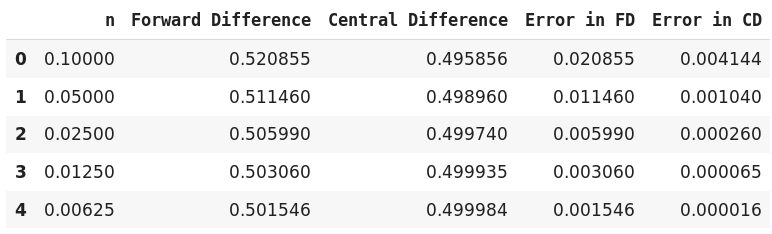
\includegraphics[width=\textwidth]{q4_1.jpg}
                \caption{plot for $cos(x)$ and $0.5+sin(x)$ }
              \end{minipage}
              \hfill
              \begin{minipage}[b]{0.45\textwidth}
                \includegraphics[width=\textwidth]{q4_2.jpg}
                \caption{plot for $f{x}$ }
              \end{minipage}
            \end{figure}
        \subsubsection{Root 1}
            \begin{figure}[!htbp]
              \centering
              \begin{minipage}[b]{0.45\textwidth}
\includegraphics[width=\textwidth]{set4_q4_data_1.png}
                \caption{Newton Rhapson }
              \end{minipage}
              \hfill
              \begin{minipage}[b]{0.45\textwidth}
                \includegraphics[width=\textwidth]{set4_q23_f_c_1.jpg}
                \caption{plot for $f(x)$}
              \end{minipage}
            \end{figure}
           \Large{Here,we can see that the root is near 1.Thus we start with x=1.\\Newton Rhapson converges faster than the bisection method.}
        \newpage
        %%%%%%%%%%%%%%%%%%%%%%%%%%%%%%%%%%%%%%%%%%%%%%%%%%%%%%%%%%%%%%%%%%%%
         \subsection{Determine both the real roots of  $f(x)=x- e^{-x}$}
            \begin{figure}[!htbp]
              \centering
              \begin{minipage}[b]{0.45\textwidth}
                \includegraphics[width=\textwidth]{q5_1.jpg}
                \caption{ for $x$ and $e^{-x}$ }
              \end{minipage}
              \hfill
              \begin{minipage}[b]{0.45\textwidth}
                \includegraphics[width=\textwidth]{q5_2.jpg}
                \caption{plot for $f{x}$}
              \end{minipage}
            \end{figure}
        \subsubsection{Root 1}
             \begin{figure}[!htbp]
              \centering
              \begin{minipage}[b]{0.45\textwidth}
\includegraphics[width=\textwidth]{set4_q5_data_1.png}
                \caption{Newton Rhapson }
              \end{minipage}
              \hfill
              \begin{minipage}[b]{0.45\textwidth}
                \includegraphics[width=\textwidth]{set4_q24_f_c_1.jpg}
                \caption{plot for $f(x)$}
              \end{minipage}
            \end{figure}
            \Large{Here,we can see that the root is near 1.Thus we start with x=1.\\Newton Rhapson converges faster than the bisection method.}
        \newpage
        %%%%%%%%%%%%%%%%%%%%%%%%%%%%%%%%%%%%%%%%%%%%%%%%%%%%%%%%%%%%%%%%%%%%%%%%%%%%%%%%%%%%%%%%%%%%%%%%%
        \subsection{Determine two smallest positive real roots of $f(x)=sin(x)-e^{-x}$}
            \begin{figure}[!htbp]
              \centering
              \begin{minipage}[b]{0.45\textwidth}
                \includegraphics[width=\textwidth]{q6_1.jpg}
                \caption{plot for $sin(x)$ and $e^{-x}$}
              \end{minipage}
              \hfill
              \begin{minipage}[b]{0.45\textwidth}
                \includegraphics[width=\textwidth]{q6_2.jpg}
                \caption{plot for $f(x)$ }
              \end{minipage}
            \end{figure}
        \subsubsection{Root 1}
            \begin{figure}[!htbp]
              \centering
              \begin{minipage}[b]{0.45\textwidth}
\includegraphics[width=\textwidth]{set4_q6_data_1.png}
                \caption{Newton Rhapson }
              \end{minipage}
              \hfill
              \begin{minipage}[b]{0.45\textwidth}
                \includegraphics[width=\textwidth]{set4_q25_f_c_1.jpg}
                \caption{plot for $f(x)$}
              \end{minipage}
            \end{figure}
            \Large{Here,we can see that the root is near 1.Thus we start with x=1.\\Newton Rhapson converges faster than the bisection method.}
            \newpage
            \subsubsection{Root 2}
             \begin{figure}[!htbp]
              \centering
              \begin{minipage}[b]{0.45\textwidth}
\includegraphics[width=\textwidth]{set4_q6_data_2.png}
                \caption{Newton Rhapson }
              \end{minipage}
              \hfill
              \begin{minipage}[b]{0.45\textwidth}
                \includegraphics[width=\textwidth]{set4_q25_f_c_2.jpg}
                \caption{plot for $f(x)$}
              \end{minipage}
            \end{figure}
            \Large{Here,we can see that the root is near 4.Thus we start with x=4.\\Newton Rhapson converges faster than the bisection method.}
        \newpage
        
        %%%%%%%%%%%%%%%%%%%%%%%%%%%%%%%%%%%%%%%%%%%%%%%%%%%%%%%%%%%%%%%%%%%%%%%%%%%%%%%%%%%%%%%%%%%
        
        \subsection{Determine smallest positive real roots of $x^3 -2x -2=0 $}
            \begin{figure}[!htbp]
              \centering
              \begin{minipage}[b]{0.45\textwidth}
                \includegraphics[width=\textwidth]{q7_1.jpg}
                \caption{plot for $x^3$ and $ 2x+2$}
              \end{minipage}
              \hfill
              \begin{minipage}[b]{0.45\textwidth}
                \includegraphics[width=\textwidth]{q7_2.jpg}
                \caption{plot for $f(x)$}
              \end{minipage}
            \end{figure}
        \subsubsection{Root 1}
             \begin{figure}[!htbp]
              \centering
              \begin{minipage}[b]{0.45\textwidth}
\includegraphics[width=\textwidth]{set4_q7_data_1.png}
                \caption{Newton Rhapson }
              \end{minipage}
              \hfill
              \begin{minipage}[b]{0.45\textwidth}
                \includegraphics[width=\textwidth]{set4_q26_f_c_1.jpg}
                \caption{plot for $f(x)$}
              \end{minipage}
            \end{figure}
            \Large{Here,we can see that the root is near 2.5 .Thus we start with x=2.5.\\Newton Rhapson converges faster than the bisection method.}
            \newpage
            
            
            %%%%%%%%%%%%%%%%%%%%%%%%%%%%%%%%%%%%%%%%%%%%%%%%%%%%%%%%%%%%%%%%%%%%%%%%%%%%%%%%%%%%%%%%%%
         \subsection{Determine all real roots of $f(x)=x^4 - x-1$}
            \begin{figure}[!htbp]
              \centering
              \begin{minipage}[b]{0.45\textwidth}
                \includegraphics[width=\textwidth]{q8_1.jpg}
                \caption{plot for $x^4$ and $ x+1$ }
              \end{minipage}
              \hfill
              \begin{minipage}[b]{0.45\textwidth}
                \includegraphics[width=\textwidth]{q8_2.jpg}
                 \caption{plot for $f(x)$}
              \end{minipage}
            \end{figure}
        \subsubsection{Root 1}
            \begin{figure}[!htbp]
              \centering
              \begin{minipage}[b]{0.45\textwidth}
\includegraphics[width=\textwidth]{set4_q8_data_1.png}
                \caption{Newton Rhapson }
              \end{minipage}
              \hfill
              \begin{minipage}[b]{0.45\textwidth}
                \includegraphics[width=\textwidth]{set4_q27_f_c_1.jpg}
                \caption{plot for $f(x)$}
              \end{minipage}
            \end{figure}
            \Large{Here,we can see that the root is near 1.5 .Thus we start with x=1.5.\\Newton Rhapson converges faster than the bisection method.}
            \newpage
            \subsubsection{Root 2}
             \begin{figure}[!htbp]
              \centering
              \begin{minipage}[b]{0.45\textwidth}
\includegraphics[width=\textwidth]{set4_q8_data_2.png}
                \caption{Newton Rhapson }
              \end{minipage}
              \hfill
              \begin{minipage}[b]{0.45\textwidth}
                \includegraphics[width=\textwidth]{set4_q27_f_c_2.jpg}
                \caption{plot for $f(x)$}
              \end{minipage}
            \end{figure}
             \Large{Here,we can see that the root is near 0 .Thus we start with x=0.\\Newton Rhapson converges faster than the bisection method.}
            \newpage
            
            
            
            %%%%%%%%%%%%%%%%%%%%%%%%%%%%%%%%%%%%%%%%%%%%%%%%%%%%%%%%%%%%%%%%%%%%%%%%%%%%%%%%%%%%%%%%%%%%
    \subsection{Determine largest real root of $f(x)=e^x-x-2$}
            \begin{figure}[!htbp]
              \centering
              \begin{minipage}[b]{0.45\textwidth}
                \includegraphics[width=\textwidth]{q9_1.jpg}
                 \caption{plot for $e^x$ and $ x+2$ }
              \end{minipage}
              \hfill
              \begin{minipage}[b]{0.45\textwidth}
                \includegraphics[width=\textwidth]{q9_2.jpg}
                \caption{plot for $f(x)$}
              \end{minipage}
            \end{figure}
        \subsubsection{Root 1}
            \begin{figure}[!htbp]
              \centering
              \begin{minipage}[b]{0.45\textwidth}
\includegraphics[width=\textwidth]{set4_q9_data_1.png}
                \caption{Newton Rhapson }
              \end{minipage}
              \hfill
              \begin{minipage}[b]{0.45\textwidth}
                \includegraphics[width=\textwidth]{set4_q28_f_c_1.jpg}
                \caption{plot for $f(x)$}
              \end{minipage}
            \end{figure}
            \Large{Here,we can see that the root is near 1.Thus we start with x=1.\\Newton Rhapson converges faster than the bisection method.}
            \newpage
            %%%%%%%%%%%%%%%%%%%%%%%%%%%%%%%%%%%%%%%%%%%%%%%%%%%%%%%%%%%%%%%%%%%%%%%%%%%%
            
            \subsection{Smallest positive real root for $f(x)=1-x-sin(x)$}
            \begin{figure}[!htbp]
              \centering
              \begin{minipage}[b]{0.45\textwidth}
                \includegraphics[width=\textwidth]{q10_1.jpg}
               
                 \caption{plot for $-sin(x)$ and $ 1-x$ }
              \end{minipage}
              \hfill
              \begin{minipage}[b]{0.45\textwidth}
                \includegraphics[width=\textwidth]{q10_2.jpg}
                \caption{plot for $f(x)$}
              \end{minipage}
            \end{figure}
        \subsubsection{Root 1}
           \begin{figure}[!htbp]
              \centering
              \begin{minipage}[b]{0.45\textwidth}
\includegraphics[width=\textwidth]{set4_q10_data_1.png}
                \caption{Newton Rhapson }
              \end{minipage}
              \hfill
              \begin{minipage}[b]{0.45\textwidth}
                \includegraphics[width=\textwidth]{set4_q29_f_c_1.jpg}
                \caption{plot for $f(x)$}
              \end{minipage}
            \end{figure}
            \Large{Here, we can see that function has root near 1 . Thus we start with x= 1.\\Newton Rhapson converges faster than the bisection method.}
            \newpage
            
            %%%%%%%%%%%%%%%%%%%%%%%%%%%%%%%%%%%%%%%%%%%%%%%%%%%%%%%%%%%%%%%%%%%%%%%%%%%%%%%%%%
            \subsection{Real roots  for $f(x)=x-tan(x)$}
            \begin{figure}[!htbp]
              \centering
              \begin{minipage}[b]{0.45\textwidth}
                \includegraphics[width=\textwidth]{q11_1.jpg}
                \caption{plot for $x$ and $ tan(x)$ }
              \end{minipage}
              \hfill
              \begin{minipage}[b]{0.45\textwidth}
                \includegraphics[width=\textwidth]{q11_2.jpg}
                \caption{plot for $f(x)$}
              \end{minipage}
            \end{figure}
            
        \subsubsection{Root near 0}
        \begin{figure}[!htbp]
    \centering
      \begin{minipage}[b]{0.45\textwidth}
        \includegraphics[width=\textwidth]{set4_q210_data_1.png}
                \caption{Newton Rhapson Table }
              \end{minipage}
              \hfill
              \begin{minipage}[b]{0.45\textwidth}
                \includegraphics[width=\textwidth]{set4_theory_q210_f_c_44.jpg}
                \caption{plot for $f(x)$}
              \end{minipage}
            \end{figure}
            \large{Here, we can see that the root looks to be near to x= 4.4.Newton Rhapson converges faster than the bisection method.}
            \newpage
            
    \subsubsection{Root near to $x=100$}
    \begin{figure}[!htbp]
    \centering
      \begin{minipage}[b]{0.45\textwidth}
        \includegraphics[width=\textwidth]{set4_q210_data_2.png}
                \caption{Newton Rhapson Table }
              \end{minipage}
              \hfill
              \begin{minipage}[b]{0.45\textwidth}
                \includegraphics[width=\textwidth]{set4_theory_q210_f_c_98.jpg}
                \caption{plot for $f(x)$}
              \end{minipage}
            \end{figure}
             \large{Here, we can see that the root looks to be near to x= 98.945.Newton Rhapson converges faster than the bisection method.}
                \newpage
    \subsection{Roots for $f(x)=a(1-x)x$}
        
     \begin{figure}[!htbp]
          \centering
          \begin{minipage}[b]{0.45\textwidth}
\includegraphics[width=\textwidth]{theory_q3_1.jpg}
            \caption{function with a=1}
          \end{minipage}
          \hfill
          \begin{minipage}[b]{0.45\textwidth}
        \includegraphics[width=\textwidth]{theory_q3_2.jpg}
            \caption{function with a=-1}
          \end{minipage}
        \end{figure}
    \subsubsection{when we start with x $<$0.5 with a=+1}
        \begin{figure}[!htbp]
          \centering
          \begin{minipage}[b]{0.45\textwidth}
\includegraphics[width=\textwidth]{set4_49.png}
            \caption{Newton Rhapson }
          \end{minipage}
          \hfill
          \begin{minipage}[b]{0.45\textwidth}
            \includegraphics[width=\textwidth]{set4_theory_q2_to0.jpg}
            \caption{plot for $f(x)$}
          \end{minipage}
        \end{figure}
         \begin{figure}[!htbp]
          \centering
          \begin{minipage}[b]{0.45\textwidth}
\includegraphics[width=\textwidth]{set4_499.png}
            \caption{Newton Rhapson }
          \end{minipage}
          \hfill
          \begin{minipage}[b]{0.45\textwidth}
            \includegraphics[width=\textwidth]{set4_4999.png}
            \caption{Newton Rhapson for x= 0.4999}
          \end{minipage}
        \end{figure}
        \begin{enumerate}
        \item As we make the start closer to 0.5 we can see that the newton Rhapson method tends to take more number of iterations to converge to the root.
        \item The function overshoot a lot in the initial phase when we make the starting value of x very much closer to 0.5
        
        \item Other important thing to note is that the when the value of x is kept greater than 0.5 it will always converge to 1 no matter what we do.  
        \end{enumerate}
        \newpage
    \subsubsection{when start x $>$ 0.5 and a = +1}
        \begin{figure}[!htbp]
          \centering
          \begin{minipage}[b]{0.45\textwidth}
\includegraphics[width=\textwidth]{set4_51.png}
            \caption{Newton Rhapson for x= 0.51 }
          \end{minipage}
          \hfill
          \begin{minipage}[b]{0.45\textwidth}
            \includegraphics[width=\textwidth]{set4_theory_q2_to1.jpg}
            \caption{f(c) vs iterations}
          \end{minipage}
        \end{figure}
         \begin{figure}[!htbp]
          \centering
          \begin{minipage}[b]{0.45\textwidth}
\includegraphics[width=\textwidth]{set4_501.png}
            \caption{Newton Rhapson for x= 0.501 }
          \end{minipage}
          \hfill
          \begin{minipage}[b]{0.45\textwidth}
            \includegraphics[width=\textwidth]{set4_5001.png}
            \caption{Newton Rhapson plot for x= 0.5001}
          \end{minipage}
        \end{figure}
        \begin{enumerate}
        \newpage
        \item As we make the start closer to 0.5 we can see that the newton Rhapson method tends to take more number of iterations to converge to the root.
        \item The function overshoot a lot in the initial phase when we make the starting value of x very much closer to 0.5
        \item Other important thing to note is that the when the value of x is kept less than 0.5 it will always converge to 0 no matter what we do.
        \item for the value of a =-1, we can see that the same situation arises just the polarity of the function changes.
        \end{enumerate}
        
        
        \newpage
        \subsection{Question 4:Find effect of a in the function f(x) = a+ $x(1-x)^2$}
        \begin{figure}[!htbp]
          \centering
          \includegraphics[width=\textwidth]{set4_q4_1.jpg}
            \caption{plot with different values of a }
          \end{figure}
        
        
        
    \newpage    
        \subsubsection{When $a=0$:}
        \begin{figure}[!htbp]
          \centering
          \begin{minipage}[b]{0.45\textwidth}
\includegraphics[width=\textwidth]{4_99_a0.png}
            \caption{Initial value $x_{0}$ = 0.99 }
          \end{minipage}
          \hfill
          \begin{minipage}[b]{0.45\textwidth}
            \includegraphics[width=\textwidth]{4_101_a0.png}
            \caption{Initial value $x_{0}$ = 1.01}
          \end{minipage}
        \end{figure}
         \begin{figure}[!htbp]
          \centering
          \begin{minipage}[b]{0.45\textwidth}
\includegraphics[width=\textwidth]{4_03_a0.png}
            \caption{Initial value $x_{0}$ = 0.3}
          \end{minipage}
          \hfill
        \end{figure}
 
\newpage 
 \subsubsection{When $a=0.05$:}
        \begin{figure}[!htbp]
          \centering
          \begin{minipage}[b]{0.45\textwidth}
\includegraphics[width=\textwidth]{4_99_a05.png}
            \caption{Initial value $x_{0}$ = 0.99 }
          \end{minipage}
          \hfill
          \begin{minipage}[b]{0.45\textwidth}
            \includegraphics[width=\textwidth]{4_101_a05.png}
            \caption{Initial value $x_{0}$ = 1.01}
          \end{minipage}
        \end{figure}
        
\newpage        
        \subsubsection{When $a=0.1$:}
        \begin{figure}[!htbp]
          \centering
          \begin{minipage}[b]{0.45\textwidth}
\includegraphics[width=\textwidth]{4_99_a01.png}
            \caption{Initial value $x_{0}$ = 0.99 }
          \end{minipage}
          \hfill
          \begin{minipage}[b]{0.45\textwidth}
            \includegraphics[width=\textwidth]{4_101_a01.png}
            \caption{Initial value $x_{0}$ = 1.01}
          \end{minipage}
        \end{figure}
        \large{Here, we can see that when the value of a is zero then we find two roots and when we increase the value of a then it happens that the root gets reduced to one.\\
        It can be seen that the number of iterations are very high when a=0.99 as compared to the number of iterations when a=1.01 when a is not equal to 0.}
\end{document}
